\section{Kontext}
\captionof{table}{Kontextbeschreibung}
  \begin{tabular}{| l | l | l|}
    \hline
    \textbf{Anforderungsquellen} & \textbf{Betrachtungsgegenstände} \\ \hline
    Bestehende Prozesse
    &
    {\parbox{0.7\textwidth}{
      \begin{itemize}
        \item Bestehende Dokumentation der Prozessabläufe.
        \item Dokumentation der bestehenden Software-Lösungen, falls vorhanden.
        \item Datenbankinhalte und Datenformate.
        \item Abteilungsschnittstellen bzw. Kommunkationsmethoden.
        \item Datenfluss bzw. Relevanz der verschiedenen Datenpunkten von einer Abteilung zur nächsten.
        \item Implizite bzw. eingebettete Anforderungen.
      \end{itemize}
    }}
    \\ \hline
    Abteilungsleiter
    &
    {\parbox{0.7\textwidth}{
      \begin{itemize}
        \item Vorstellungen des Endproduktes und dessen Plausibilität 
        \item Kommunikationsmedien, mit welchen die Abteilung arbeitet
        \item Priorisierung der Abläufe d.h. Businesskritische Abläufe zuerst
        \item Abteilungübergreifende Prozesse und dessen Schwachstellen
      \end{itemize}
    }}
    \\ \hline    
    Dokumentation, Fall-Archiv
    &
    {\parbox{0.7\textwidth}{
      \begin{itemize}
        \item Legale Aspekte analysieren; hätte man etwas besser machen können? 
        \item Probleme identifizieren
        \item Nicht vorhandene Dokumentation notieren
      \end{itemize}
    }}
    \\ \hline      
  \end{tabular}

%\begin{landscape}
\begin{center}
  \begin{figure}[ht]
    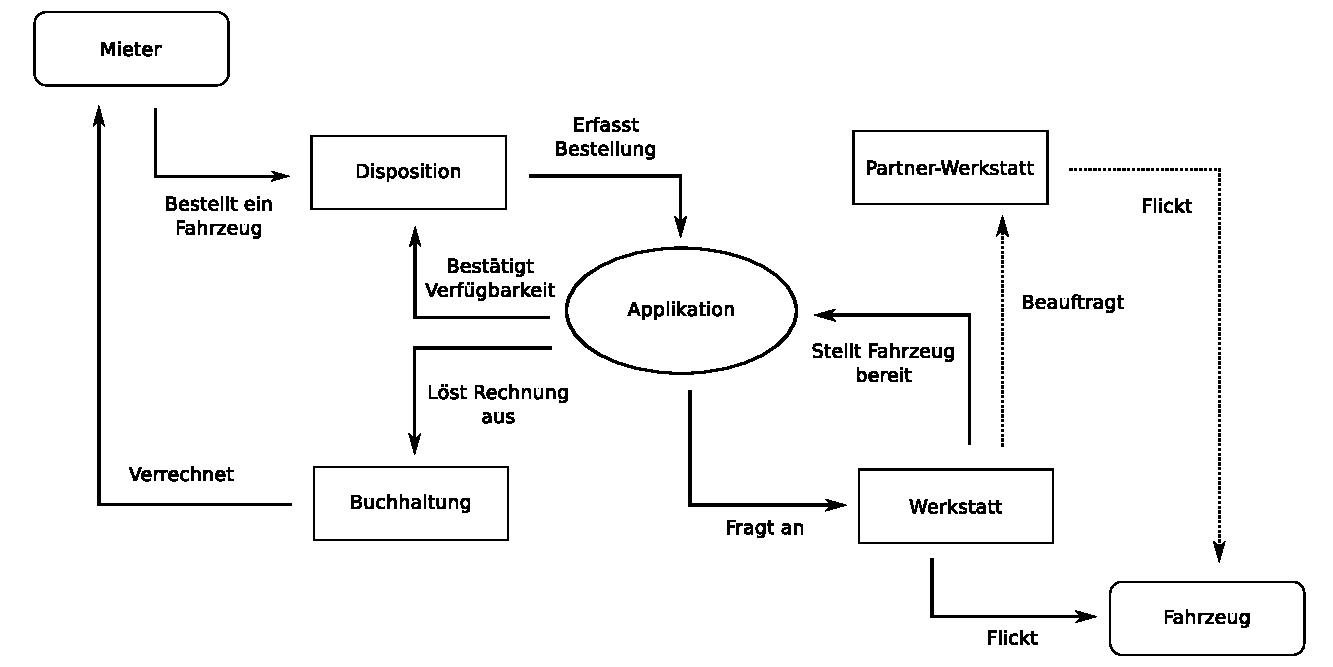
\includegraphics[width=20cm,height=16cm, angle=270]{graphics/kontextdiagramm.pdf}
    \caption{Kontextdiagramm des Endproduktes in der Nutz AG}
    \label{fig:awesome_image}
  \end{figure}
\end{center}
%\end{landscape}
